\section{The VCapsBench Benchmark}


\subsection{Overview}
Although existing benchmarks can assess the quality of VLM-generated image captions across various dimensions, as discussed in Sec.~\ref{sec:RelatedWork}, they still fall short in evaluating the fine-grained video captions produced by VLMs. To effectively measure the understanding and descriptive capabilities of VLMs across different types of video, we have constructed a large-scale high-quality benchmark VCapsBench for video caption quality evaluation.

\begin{figure*}[tp]
	\begin{minipage}[t]{1.0\linewidth}
        \centering
	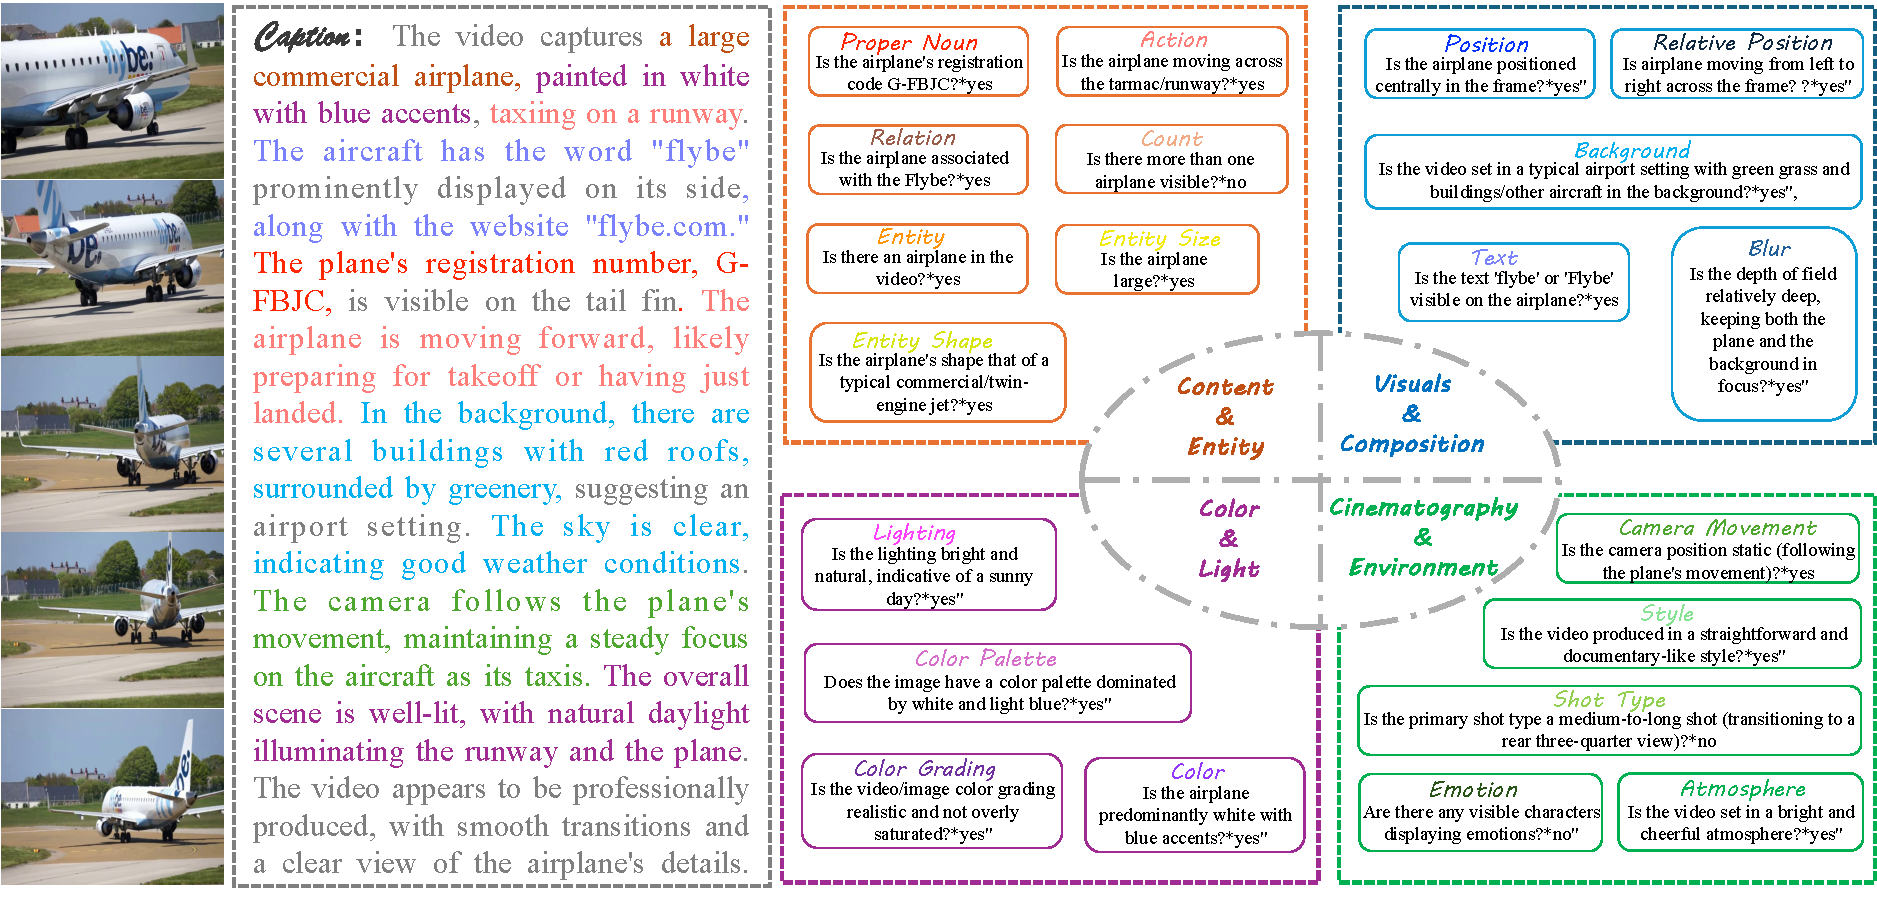
\includegraphics[width=0.95\linewidth]{imgs/method1-3.pdf}
	\caption{An example of video caption and  question-answer pairs in our VCapsBench.}
	\label{fig:fig2}
	\end{minipage}%
	\vspace{-1.0em}	
\end{figure*}

\begin{figure*}[tp]
	\begin{minipage}[t]{1.0\linewidth}
        \centering
	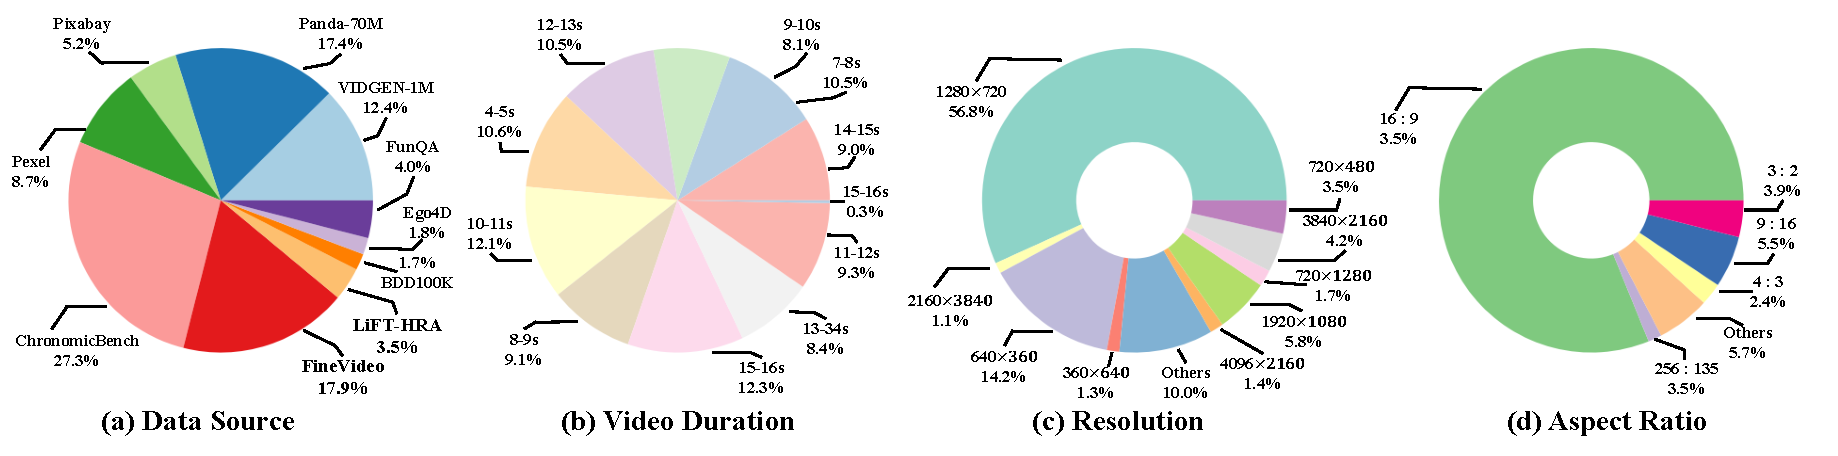
\includegraphics[width=0.95\linewidth]{imgs/method3-3.pdf}
	\caption{(a) Video source distribution; (b) Video duration distribution; (c) Video resolution distribution (d) Video aspect ratio distribution.}
	\label{fig:fig3}
	\end{minipage}%
	\vspace{-1.5em}	
\end{figure*}


\subsection{Dataset Statistics}
\textbf{Data Dimensions.} As shown in Fig.~\ref{fig:fig2}, the evaluation of video captions is organized into four primary categories: ``Content and Entity", ``Visuals and Composition" ``Color and Lighting" and ``Cinematography and Atmosphere". ``Content and Entity" includes seven subcategories, which focus on core elements like action, count, entity, entity size, entity shape, proper noun and relation. ``Visuals and Composition" is related to spatial arrangement and visual presentation, comprising five subcategories: position, relative position, text, blur, and background. ``Color and Lighting" addresses how these elements enhance mood and style, covering four subcategories: color, color palette, color grading, and lighting. Finally, ``Cinematography and Atmosphere" includes five subcategories: camera movement, shot type, style, atmosphere, and emotion, integrating filming techniques and artistic expression.  By categorizing these dimensions, it becomes easier to statistically analyze the quality of video  captions across different categories. This provides more detailed guidance for optimizing VLM's video understanding capabilities.

\textbf{Data Collection.} To fully support the caption evaluation task in video understanding and generation tasks, we prioritized  the complexity of aesthetic and content in our data collection for VCapsBench. We sourced videos from 10 publicly available datasets to ensure diversity: Panda-70M\cite{ChenSMDCJF0RYT24}, Ego4D\cite{grauman2022ego4d}, BDD100K\cite{yu2020bdd100k}, Pixabay~\cite{chensharegpt4video}, Pexel~\cite{chensharegpt4video}, VIDGEN-1M\cite{tan2024vidgen}, ChronomicBench~\cite{yuan2024chronomagic}, FineVideo~\cite{Farre2024FineVideo}, FunQA~\cite{yuan2024chronomagic}, and LiFT-HRA-20K~\cite{wang2024lift}. As illustrated in Fig.~\ref{fig:fig3}, we curated a diverse collection of 988 high-resolution videos from Panda-70M\cite{ChenSMDCJF0RYT24}, encompassing a wide range of scenes such as wildlife, cooking, sports, TV shows, gaming, and 3D rendering. These videos often contain complex content and transformations, providing a robust foundation for understanding various real-world scenarios. Additionally, we included 494 high-resolution videos from Pexels and 298 from Pixabay, both renowned for their scenic landscapes and human activities, characterized by high aesthetic quality and detailed imagery. To further ensure data diversity, we sample 1,018 videos from FineVideo\cite{Farre2024FineVideo}, which encompasses 6 major categories and 122 subcategories. Despite their lower resolution (below 640 $ \times $360), we balanced this by sampling 333 ultra-high-resolution videos (2K, 3K, and 4K) from VIDGEN-1M\cite{tan2024vidgen}, typically used for training text-to-video models due to their high detail and quality. Our collection was further enriched with videos from Ego4D\cite{grauman2022ego4d} and BDD100K\cite{yu2020bdd100k} to cover ego-centric human activities and autonomous driving scenarios, ensuring a comprehensive representation of real-world scenes.
To evaluate the VLM model's understanding of object motion and physical laws, we included 1,549 videos from ChronomicBench, spanning four main categories
(\eg, biological, artificial, meteorological, and physical) across 75 subcategories. To further diversify our dataset, we sampled 227 videos from FunQA and 200 from LiFT-HRA-20K. FunQA features human-centric content such as humorous clips, creative performances, and visual illusions, while LiFT-HRA-20K consists of synthetic video data.


As shown in Fig.~\ref{fig:fig3}, our VCapsBench dataset comprises 5,677 videos from a wide range of scenes, e.g., natural landscapes, animals, human activities, physical phenomena, games, 3D renderings, and synthetic videos (more than 100 subcategories). VCapsBench also features diverse video durations (4 to 16 seconds), resolutions (125 different resolutions), and aspect ratios (87 different ratios). This extensive collection allows for a thorough evaluation of VLM models' understanding and insight across various video types, ensuring a robust assessment of video captioning.

\begin{figure*}[thbp]
	\begin{minipage}[t]{1.0\linewidth}
        \centering
	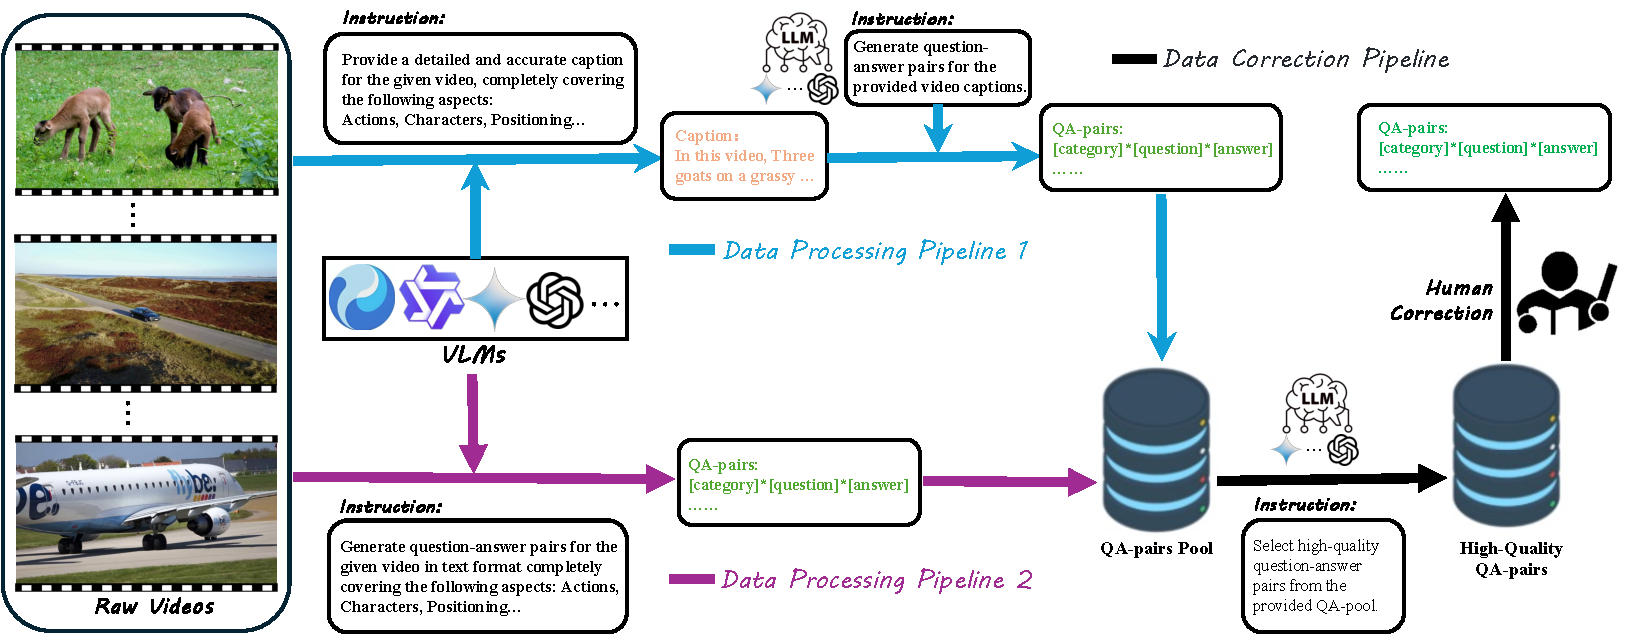
\includegraphics[width=0.9\linewidth]{imgs/method2.pdf}
	\caption{The pipeline of QA-pairs generation, which includes multiple data processing pipelines and a data correction pipeline.}
	\label{fig:fig4}
	\end{minipage}%
	\vspace{-1.0em}	
\end{figure*}

\subsection{Annotation Details}
Inspired by DPG-bench~\cite{Ella} and CapsBench~\cite{playgroundv3}, we developed a method to evaluate video caption quality using multi-dimensional question-answer pairs. Based on the raw video, we generate ``yes-no" question-answer pairs as annotations. As shown in Fig.~\ref{fig:fig4}, our ``Data Processing Pipeline" creates these pairs, which are stored in the ``QA-pairs Pool". Each pair includes a category, question, and answer, formatted as ``[category][question][answer]" for easy processing. To ensure diversity and accuracy, we designed two data production pipelines. The first one uses various VLMs, such as Geinimi, Qwen, and HunYuan, to generate detailed video captions from predefined prompts. Large Language Models (LLMs) like GPT-4, Gemini, and Qwen72B then use these captions and additional prompts to create question-answer pairs. The second approach directly utilizes VLMs to generate question-answer pairs from videos and prompts. The outputs from both pipelines are then combined into a comprehensive question-answer pool.


\begin{figure}[tp]
	\begin{minipage}[t]{1.0\linewidth}%\centering
	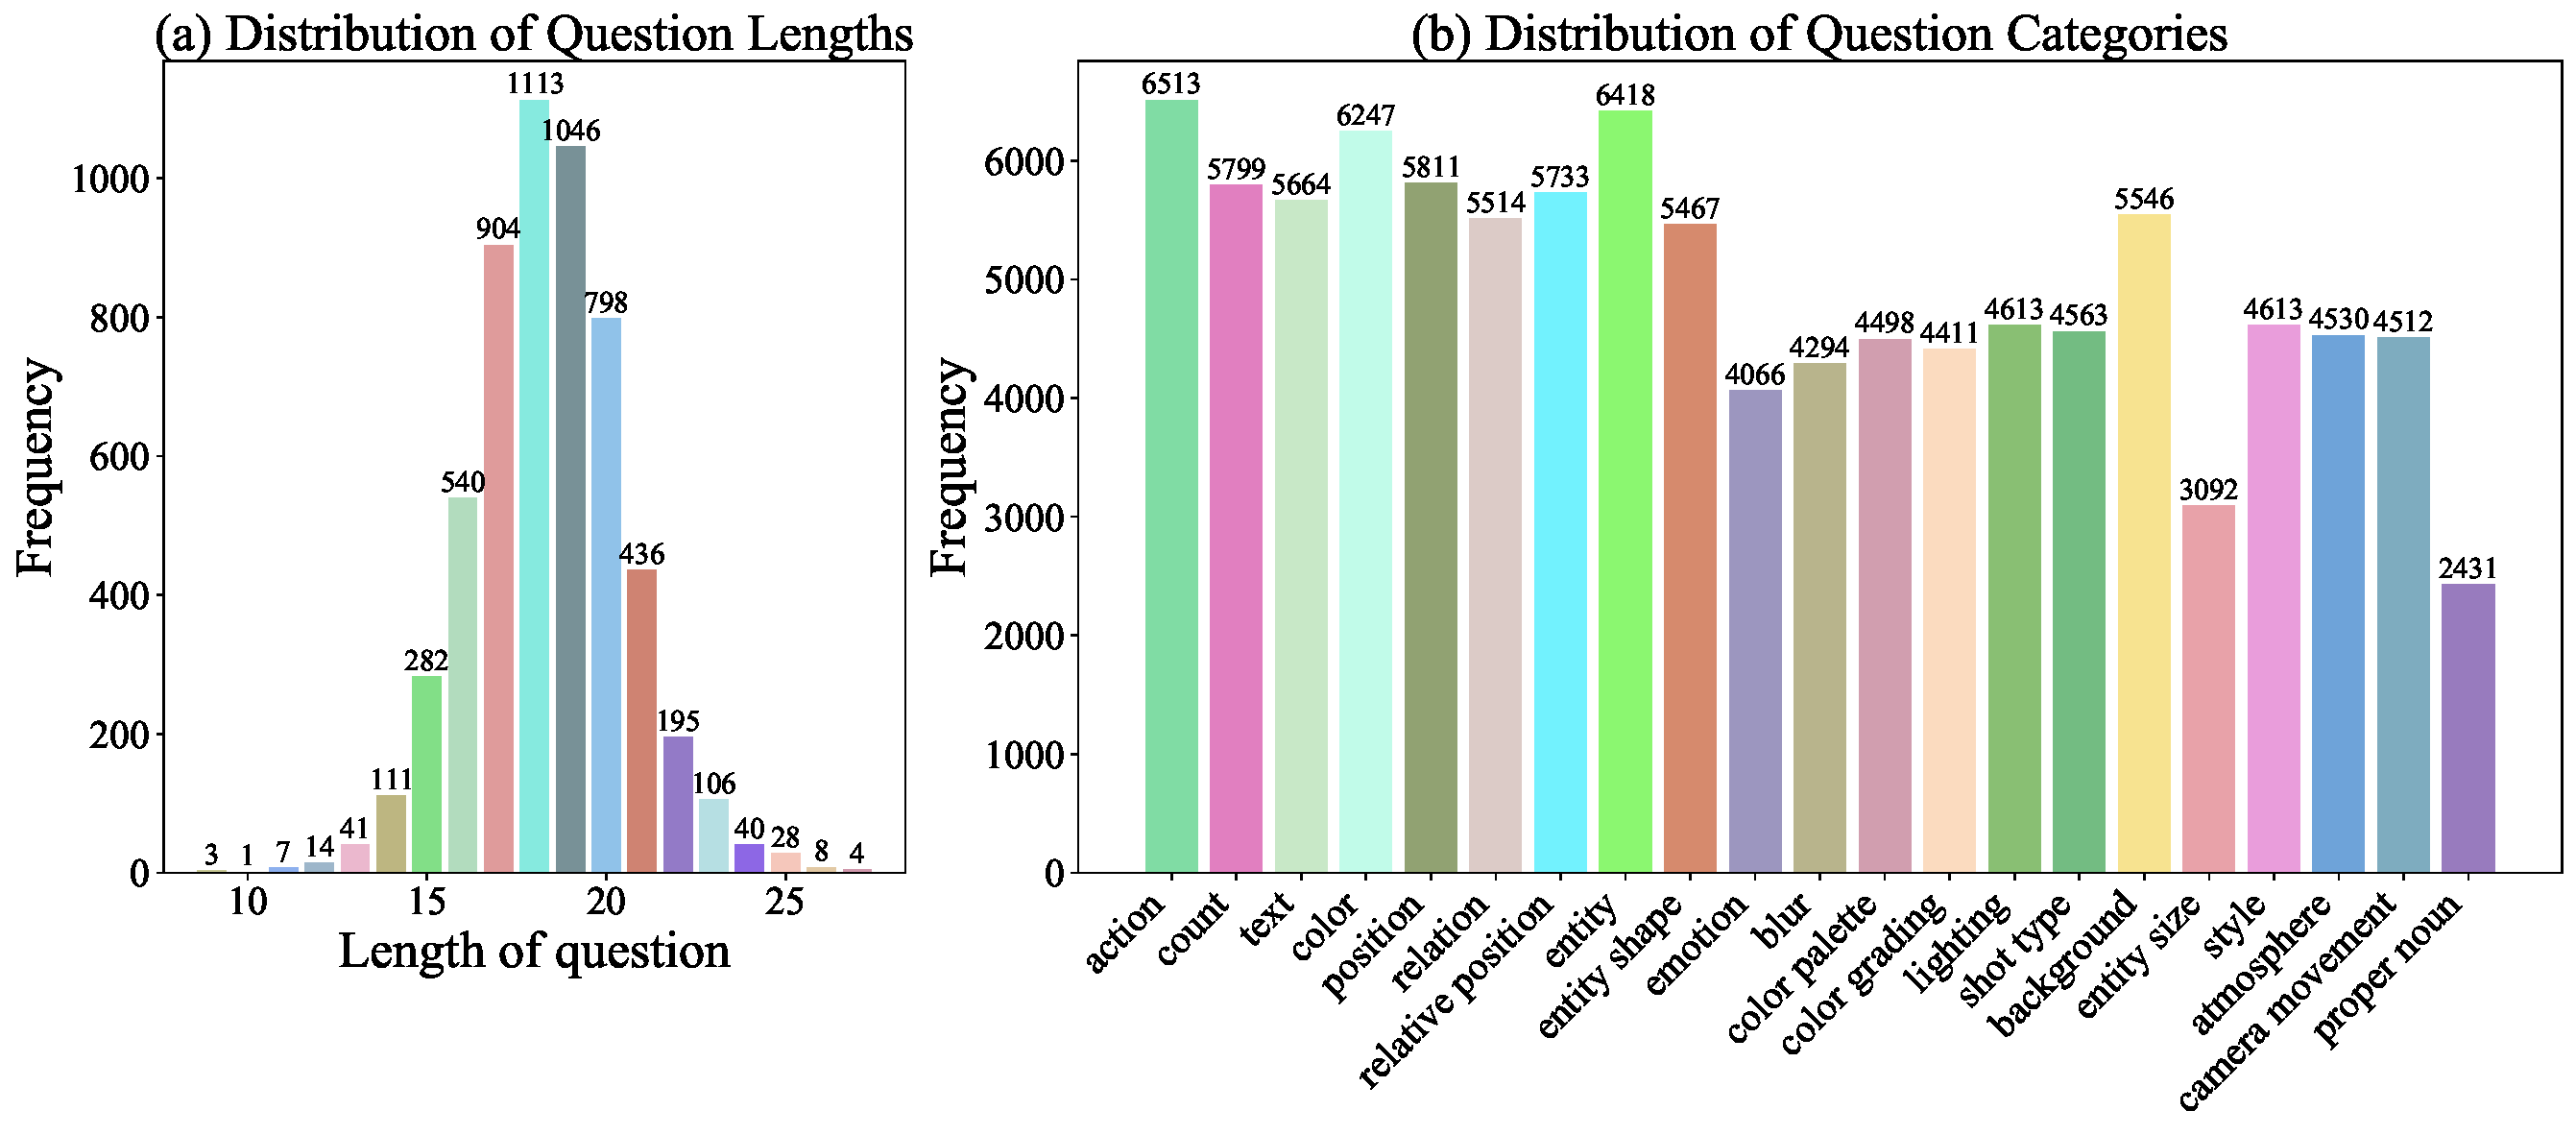
\includegraphics[width=0.9\linewidth]{imgs/qa_distribution-2.pdf}
	\caption{The question length and category distribution.}
	\label{fig:fig5}
	\end{minipage}%
	\vspace{-1.0em}	
\end{figure}

To enhance the quality of the QA-pairs, we established a data correction pipeline. This pipeline takes multiple sets of QA-pairs and captions from the same video as input and uses an advanced LLM (Gemini1.5) with predefined instructions to de-duplicate, filter, and retain high-quality QA-pairs. The instructions guide the LLM to merge similar QA-pairs, filter out those with the same question but different answers, and remove QA-pairs that appear only once, as they are likely to be invalid.



\textbf{Human Correction.} After generating high-quality candidate QA-pairs, we sample the data according to latitude to ensure that the data focuses more on important latitudes, and then conduct a final quality control process manually. Human reviewers re-examine these QA-pairs, deleting those with unreasonable or incorrect questions and correcting those with erroneous answers. Following this manual revision, we establish a benchmark (VCapsBench) consisting of 5,677 videos and 109,796 question-answer pairs. As shown in Fig.~\ref{fig:fig5}, each video contains between 10 and 27 QA-pairs, with each category comprising between 2,431 and 6,513 QA-pairs. The questions are organized into four major categories and 21 subcategories. Most answers are ``yes" providing a clear indication of correctness, while a smaller number of ``no" answers help assess whether the video captions contain hallucinations or inaccuracies.


\begin{figure*}[tp]
	\begin{minipage}[t]{1.0\linewidth}
        \centering
	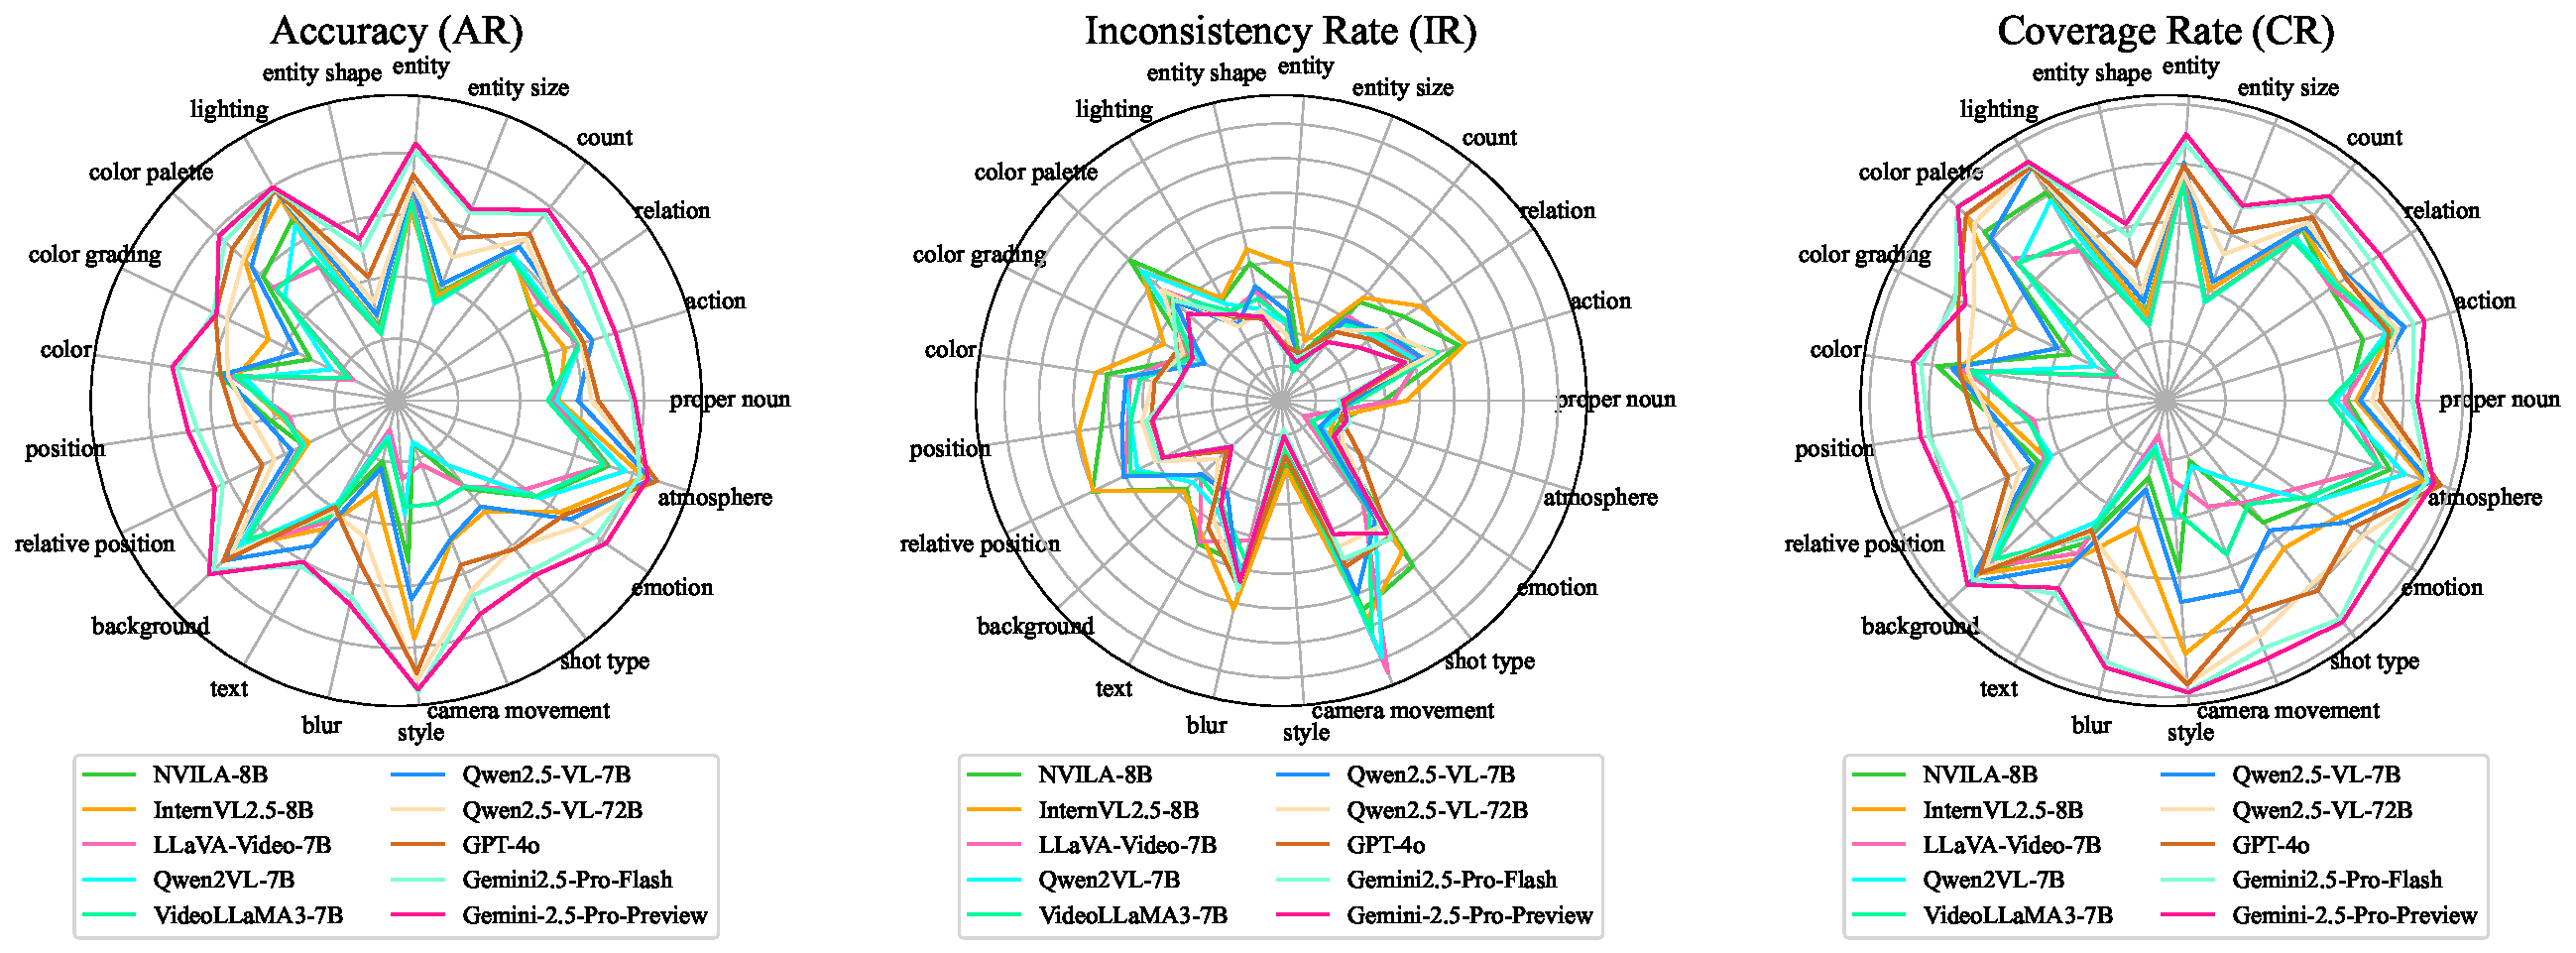
\includegraphics[width=1.0\linewidth]{imgs/radar_chart_all-New.pdf}
	\caption{Results of Gemini-2.5-Pro-Preview captioning evaluation, organized by category.}
	\label{fig:fig6}
	\end{minipage}%
	\vspace{-1.5em}	
\end{figure*}

\subsection{Captioning Evaluation}
We employ VCapsBench to evaluate video captions produced by various vision-language models (VLMs), including top proprietary models like Gemini-1.5. For each test video, an evaluation-capable VLM generates a detailed caption according to specific guidelines and an output schema. This caption, along with each question from the video's QA pairs, is fed into a Large Language Model (LLM). As shown in Fig.~\ref{fig:fig1}, the LLM responds to each question based on the caption, providing answers in the format ``[answer], [reason]." We instruct the LLMs to assess the caption in the following three scenarios:

\begin{itemize}
    \item \textbf{Positive:} The caption accurately describes the relevant content, and the LLM's response aligns with the answer.
    
    \item \textbf{Negative:} The caption mentions the relevant content, but the LLM's response does not align with the answer.
    
    \item \textbf{Unanswerable:} The caption does not involve the relevant content for the dimension.
\end{itemize}

To comprehensively evaluate the quality of the captions, we developed three metrics tailored to these scenarios. The quality of the captions is evaluated using the following measure:

\begin{equation}
AR = \dfrac{N(\text{Positive})}{N(\text{All})},
\end{equation}

\begin{equation}
IR = \dfrac{N(\text{Negative})}{N(\text{Positive}) + N(\text{Negative})},
\end{equation}

\begin{equation}
CR = \dfrac{N(\text{Positive}) + N(\text{Negative})}{N(\text{All})},
\end{equation}


\textbf{Accuracy (AR):} This metric evaluates the percentage of ``Positive" responses, indicating that the caption correctly describes the relevant content and aligns with the LLM's response. A higher AR signifies a more accurate and reliable caption, reflecting better quality in the LLM's outputs.

\textbf{Inconsistency Rate (IR):} This metric measures the percentage of ``Negative" responses among all responses that reference the relevant content (both ``Positive" and ``Negative"). A lower IR denotes a more accurate caption, indicating that when the caption involves relevant content, it is more likely to be consistent with the real video content.

\textbf{Coverage Rate (CR):} This metric evaluates the total percentage of "Positive" and ``Negative" responses, reflecting whether the caption contains the relevant content, independent of the LLM's response consistency. A higher CR indicates a superior caption richness, as it suggests that the caption encompasses a greater amount of pertinent content from the video.


\begin{table*}[!t]
\renewcommand{\arraystretch}{0.6}
\caption{The accuracy (AR), inconsistency rate (IR), and coverage rate (CR) of VLM methods on all dimensions, where Gemini-2.5-Pro-Preview as a TextQA expert. The symbol ``$\uparrow$"  indicates that the larger the value, the better; The symbol ``$\downarrow$" indicates that the smaller the value, the better.}
\label{tab:results_1}
\resizebox{\textwidth}{!}{%
\begin{tabular}{@{}ll|cccccccccccc@{}}
\toprule
 &\multirow{3}{*}{Methods}& \multicolumn{7}{c|}{Content \& Entity}& \multicolumn{4}{c}{Color \&  Light}\\
 \cline{3-13} 
 &  & \begin{tabular}[c]{@{}c@{}}\small Proper\\ \small Noun\end{tabular} & \begin{tabular}[c]{@{}c@{}}Action\end{tabular} & \begin{tabular}[c]{@{}c@{}}Relation
\end{tabular} & \begin{tabular}[c]{@{}c@{}}Count
\end{tabular} & Entity  & \begin{tabular}[c]{@{}c@{}}\small Entity\\ \small Size\end{tabular} & \multicolumn{1}{c|}{\begin{tabular}[c]{@{}c@{}}\small Entity\\ \small Shape\end{tabular} }
&\begin{tabular}[c]{@{}c@{}}Lighting
\end{tabular} & \begin{tabular}[c]{@{}c@{}}\small Color \\ \small Palette \end{tabular} & \begin{tabular}[c]{@{}c@{}}\small Color\\ \small Grading
\end{tabular} & \begin{tabular}[c]{@{}c@{}}Color
\end{tabular}  \\ \midrule
\multirow{8}{*}{\rotatebox{90}{AR}$\Bigg\uparrow$} 
% & Qwen2VL-72B & 36.53 & 43.15 & 38.62 & 42.72 & 49.51 & 22.29 & \multicolumn{1}{c|}{14.45} & 50.81 & 37.25 & 20.20 &35.08  \\
& LLaVA-Video-7B & 50.45 & 61.6 & 55.98 & 59.47 & 67.68 & 34.22 & \multicolumn{1}{c|}{22.27} & 49.83 & 53.92 & 15.52 &\multicolumn{1}{c|}{53.96} \\
& Qwen2VL-7B & 51.98 & 62.11 & 58.08 & 60.27 & 65.35 & 33.60 & \multicolumn{1}{c|}{22.62} & 65.38 & 49.11 & 23.33 &\multicolumn{1}{c|}{49.49} \\ 
& VideoLLaMA3-7B & 48.97 & 66.29 & 57.12 & 58.94 & 65.30 & 34.45 & \multicolumn{1}{c|}{22.07} & 53.14 & 52.92 & 35.67 &\multicolumn{1}{c|}{56.48}\\
& NVILA-8B & 52.12 & 50.77 & 52.74 & 60.39 & 64.90 & 37.36 & \multicolumn{1}{c|}{24.21} & 67.37 & 58.71 & 30.74 &\multicolumn{1}{c|}{58.27} \\ 
& InternVL2.5-8B & 52.55 & 57.07 & 53.10 & 60.18 & 62.07 & 36.49 & \multicolumn{1}{c|}{23.04} & 74.97 & 66.81 & 45.82 &\multicolumn{1}{c|}{52.04} \\
& Qwen2.5VL-7B & 58.73 & 66.29 & 61.23 & 63.69 & \textbf{70.13} & 40.38 & \multicolumn{1}{c|}{28.28} & 79.58 & 63.81 & 35.67 &\multicolumn{1}{c|}{56.48} \\ 
& Qwen2.5-VL-72B & 63.14 &62.77 &60.25 &66.74 & 49.81 &69.71& \multicolumn{1}{c|}{32.72} & \textbf{79.99} &67.46 &60.77 &\multicolumn{1}{c|}{55.09} \\ 

& GPT-4o &65.28 &63.39 &61.81 &69.04 &56.51 &73.16 &\multicolumn{1}{c|}{40.9} &78.41 &72.27 &64.86 &\multicolumn{1}{c|}{57.56} \\ 
& Gemini2.5-Pro-Flash &76.19 &70.76 &72.23 &76.94 &65.26 &80.91 & \multicolumn{1}{c|}{49.66} &79.01 &75.68 &\textbf{65.56} &\multicolumn{1}{c|}{71.65} \\ 

& Gemini-2.5-Pro-Preview &\textbf{77.14} &\textbf{74.13} &\textbf{75.35} &\textbf{78.72} &66.43 &\textbf{83.33} & \multicolumn{1}{c|}{\textbf{53.53}} &79.67 &\textbf{78.24} &64.47 &\multicolumn{1}{c|}{\textbf{73.27}} \\ 

% & Gemini-1.5 & \textbf{86.28} & \textbf{90.29} & \textbf{89.51} & \textbf{80.75} & \textbf{94.99} & \textbf{69.05} & \multicolumn{1}{c|}{\textbf{59.05}} & \textbf{96.20} & \textbf{97.39} & \textbf{74.90}&\textbf{86.28}\\ 
\midrule
\multirow{8}{*}{\rotatebox{90}{IR}$\Bigg\downarrow$} 
% & Qwen2VL-72B & 12.78 & 20.81 & 16.37 & 14.88 & 9.37 & 4.97 & \multicolumn{1}{c|}{14.25} & 13.79 & 25.39 & 11.37 & 22.29 \\
& LLaVA-Video-7B & 16.21 & 20.98 & 16.96 & 15.54 & 10.82 & 5.80 & \multicolumn{1}{c|}{16.32} & 14.44 & 23.46 & 15.37 & \multicolumn{1}{c|}{22.08}\\
& Qwen2VL-7B & 9.22 & 20.15 & 16.42 & 14.11 & 11.16 & 5.47 & \multicolumn{1}{c|}{13.52} & 16.14 & 27.44 & 12.60 & \multicolumn{1}{c|}{22.84} \\
& VideoLLaMA3-7B & 11.20 & 23.64 & 16.94 & 14.49 & 11.42 & \textbf{4.49} & \multicolumn{1}{c|}{15.09} & 14.95 & 22.30  & 14.25 & \multicolumn{1}{c|}{20.62} \\
& NVILA-8B & 14.81 & 26.92 & 21.50 & 18.19 & 15.49 & 6.94  & \multicolumn{1}{c|}{20.37} &16.89 & 29.80 & 14.37 & \multicolumn{1}{c|}{25.46} \\
& InternVL2.5-8B & 18.10 & 27.82 & 24.24 & 19.00 & 19.50 & 9.19 & \multicolumn{1}{c|}{22.42} & 17.18 & 27.38 & 18.80 & \multicolumn{1}{c|}{27.06} \\
& Qwen2.5VL-7B & 10.26 & 21.20 & 17.72 & 14.86 & 12.81 & 6.03 & \multicolumn{1}{c|}{16.95} & 12.60 &  21.00 & \textbf{12.34} & \multicolumn{1}{c|}{22.65} \\

& Qwen2.5-VL-72B &8.97 &23.08 &17.97 &12.94 &5.99 &9.58 & \multicolumn{1}{c|}{13.35} &\textbf{12.35} &23.47 &15.69 &\multicolumn{1}{c|}{18.76} \\ 
& GPT-4o &9.53 &19.36 &15.71 &12.66 &7.28 &7.96 & \multicolumn{1}{c|}{\textbf{12.1}} &13.95 &21.54 &16.69 &\multicolumn{1}{c|}{18.5} \\ 
& Gemini2.5-Pro-Flash &\textbf{8.23} &19.04 &\textbf{13.55} &10.91 &6.63 &7.0 & \multicolumn{1}{c|}{12.56} &14.22 &21.4 &16.83 &\multicolumn{1}{c|}{\textbf{14.4}}  \\

& Gemini-2.5-Pro-Preview &8.95 &\textbf{18.7} &13.59 &\textbf{10.79} &\textbf{5.92} &7.54 & \multicolumn{1}{c|}{12.42} &14.36 &\textbf{18.42} &14.23 &\multicolumn{1}{c|}{15.21}\\ 


% & Gemini-1.5 & \textbf{4.73} & \textbf{8.18} & \textbf{7.02} & \textbf{9.02} & \textbf{3.89} &\textbf{3.75}  & \multicolumn{1}{c|}{\textbf{7.07}} & \textbf{3.17} & \textbf{2.32} & \textbf{6.71} & \textbf{8.71}\\ 
 \midrule
\multirow{8}{*}{\rotatebox{90}{CR}$\Bigg\uparrow$} 
% & Qwen2VL-72B & 41.89 & 54.48 & 46.18 & 50.19 & 54.63 & 23.46 & \multicolumn{1}{c|}{16.85} & 58.94 & 49.92 & 22.79 & 45.14  \\
& LLaVA-Video-7B & 60.21 & 77.95 & 67.41 & 70.41 & 75.89 & 36.33 & \multicolumn{1}{c|}{26.62} & 58.24 & 70.45 & 18.33 &\multicolumn{1}{c|}{69.26}  \\
& Qwen2VL-7B & 57.17 & 77.79 & 69.50 & 70.20 & 73.56 & 35.55 & \multicolumn{1}{c|}{26.26} & 77.97 & 67.68 & 26.69 &\multicolumn{1}{c|}{64.15} \\ 
& VideoLLaMA3-7B & 55.14 & 81.34 & 68.77 & 68.92 & 73.72 & 36.07 & \multicolumn{1}{c|}{26.00} & 62.48 & 68.10 & 19.76 &\multicolumn{1}{c|}{66.53}  \\
& NVILA-8B & 61.19 & 69.48 & 67.19 & 73.82 & 76.80 & 40.15 & \multicolumn{1}{c|}{30.41} & 81.06 & 83.63 & 35.89 &\multicolumn{1}{c|}{78.17} \\
& InternVL2.5-8B & 64.17 & 79.06 & 70.08 & 74.30 & 77.11 & 40.15 & \multicolumn{1}{c|}{29.68} & 90.52 & 92.00 & 56.43 &\multicolumn{1}{c|}{71.34}  \\
& Qwen2.5VL-7B & 65.44 & 84.12 & 74.43 & 74.80 & \textbf{80.44} & 42.97 & \multicolumn{1}{c|}{34.06} & 91.05 & 80.78 & 40.69 & \multicolumn{1}{c|}{73.03}\\ 

& Qwen2.5-VL-72B &69.36 &81.6 &73.45 &76.66 &52.98 &77.1 & \multicolumn{1}{c|}{37.76} &91.27 &88.15 &72.08 &\multicolumn{1}{c|}{67.81} \\ 

& GPT-4o &72.16 &78.61 &73.34 &79.05 &60.95 &79.48 & \multicolumn{1}{c|}{46.53} &91.11 &92.12 &77.85 &\multicolumn{1}{c|}{70.62} \\ 
& Gemini2.5-Pro-Flash &83.03 &87.4 &83.55 &86.36 &69.9 &86.99 &\multicolumn{1}{c|}{56.79} &92.11 &\textbf{96.28} &\textbf{78.83} &\multicolumn{1}{c|}{83.7} \\ 
& Gemini-2.5-Pro-Preview &\textbf{84.72} &\textbf{91.17} &\textbf{87.2} &\textbf{88.25} &70.61 &\textbf{90.12} &\multicolumn{1}{c|}{\textbf{61.12}} &\textbf{93.03} &95.9 &75.17 &\multicolumn{1}{c|}{\textbf{86.41}} \\ 


% & Gemini-1.5 & \textbf{90.56} & \textbf{98.33} & \textbf{96.27} & \textbf{88.75} & \textbf{98.82} & \textbf{71.74} & \multicolumn{1}{c|}{\textbf{63.54}} & \textbf{99.34} & \textbf{99.71} & \textbf{80.28} &\textbf{94.51} \\ 
 \bottomrule
 \toprule
 &\multirow{3}{*}{Methods}& \multicolumn{5}{c|}{Visuals \& Composition}& \multicolumn{5}{c|}{Cinematography  \& Environment}\\
 \cline{3-13} 
 &  & Position & \begin{tabular}[c]{@{}c@{}}\small Relative\\ \small Position\end{tabular} & Background &Text & \multicolumn{1}{c|}{Blur} & Style & \begin{tabular}[c]{@{}c@{}}\small Camera \\ \small Movement\end{tabular} & \begin{tabular}[c]{@{}c@{}}Shot Type\end{tabular} & \begin{tabular}[c]{@{}c@{}}Emotion\end{tabular} & \multicolumn{1}{c|}{Atmosphere} & \color{red}\textbf{ALL}\\ \midrule
\multirow{8}{*}{\rotatebox{90}{AR}$\Bigg\uparrow$} 
% & Qwen2VL-72B & 22.85 & 21.29 & 48.67 & 26.77 & \multicolumn{1}{c|}{10.43} & 35.10 & 16.17 & 21.71 & 35.94 & \multicolumn{1}{c|}{52.14} &33.01 \\ 
& LLaVA-Video-7B & 34.91 & 34.31 & 69.57 & 45.47 & \multicolumn{1}{c|}{9.61} & 25.30 & 22.17 & 35.47 & 50.78 & \multicolumn{1}{c|}{70.64} &45.11 \\
& Qwen2VL-7B & 36.69 & 33.10 & 69.45 & 38.51 & \multicolumn{1}{c|}{11.72} & 36.86 & 14.33 & 26.76 & 55.96 & \multicolumn{1}{c|}{77.41} &45.75\\ 
& VideoLLaMA3-7B & 36.45 & 33.80 & 65.86 & 43.73 & \multicolumn{1}{c|}{13.09} & 34.51 & 35.75 & 35.51 & 54.84 & \multicolumn{1}{c|}{70.33} &46.13 \\
& NVILA-8B & 41.44 & 33.31 & 69.79 & 42.32 & \multicolumn{1}{c|}{20.04} & 52.29 & 14.81 & 36.54 & 55.36 & \multicolumn{1}{c|}{71.74} &47.99  \\
& InternVL2.5-8B & 37.55 & 31.37 & 69.44 & 47.99 & \multicolumn{1}{c|}{30.36} & 77.08 & 48.61 & 45.90 & 64.00 & \multicolumn{1}{c|}{83.67} &53.30  \\
 & Qwen2.5VL-7B & 43.06 & 37.43 & 76.03 & 54.13 & \multicolumn{1}{c|}{22.33} & 64.43 & 48.10 & 43.79 & 68.12 & \multicolumn{1}{c|}{86.17} &56.03 \\ 
& Qwen2.5-VL-72B & 46.93 &43.73 &72.59 &41.27 & \multicolumn{1}{c|}{45.37} & 90.53 &66.07 &60.76 &71.97 & \multicolumn{1}{c|}{87.94} &61.20 \\
& GPT-4o &52.45 &48.08 &76.35 &39.77 & \multicolumn{1}{c|}{53.33} &88.29 &57.03 &61.35 &65.64 & \multicolumn{1}{c|}{\textbf{88.16}} &63.08 \\


& Gemini2.5-Pro-Flash &65.03 &62.2 &80.47 &\textbf{61.95} &
\multicolumn{1}{c|}{65.09} &\textbf{94.48} &67.67 &70.17 &77.94 & \multicolumn{1}{c|}{82.5} &71.77 \\
& Gemini-2.5-Pro-Preview &\textbf{67.98} &\textbf{65.12} &\textbf{82.55} &60.19 & \multicolumn{1}{c|}{\textbf{67.56}} &93.63 &\textbf{74.12} &\textbf{72.08} &\textbf{82.03} & \multicolumn{1}{c|}{85.09} &\color{red}\textbf{73.88} \\

 
 % & Gemini-1.5 & \textbf{83.91} & \textbf{78.63} & \textbf{94.78} & \textbf{79.22} & \multicolumn{1}{c|}{\textbf{80.19}} &\textbf{98.02} & \textbf{77.41} & \textbf{81.89} & \textbf{95.76} & \multicolumn{1}{c|}{\textbf{85.93}} &\textbf{84.99} \\ 
 \midrule
\multirow{8}{*}{\rotatebox{90}{IR}$\Bigg\downarrow$} 
% & Qwen2VL-72B & 23.32 & 22.62 & 16.36 & 29.48 & \multicolumn{1}{c|}{27.79} & 7.13 & 33.58 & 21.57 & 7.25  & \multicolumn{1}{c|}{7.72} &17.04 \\
& LLaVA-Video-7B & 22.41 & 25.02 & 15.83 & 23.50 & \multicolumn{1}{c|}{\textbf{20.77}} & 5.52 & 42.21 & \textbf{18.96} & \textbf{3.96}  & \multicolumn{1}{c|}{\textbf{6.28}} & 17.46 \\
& Qwen2VL-7B & 21.94 & 23.07 & 17.36 & 18.34 & \multicolumn{1}{c|}{25.41} & 6.45 & 39.83 & 21.71 & 7.24 & \multicolumn{1}{c|}{8.21} &16.79 \\
& VideoLLaMA3-7B & 22.05 & 24.13 & 16.06 & 17.30 & \multicolumn{1}{c|}{23.47} & 6.75 & 35.85 & 20.33 & 5.36  & \multicolumn{1}{c|}{6.83} & 17.09\\
& NVILA-8B & 26.26 & 30.28 & 18.66 & 23.91 & \multicolumn{1}{c|}{24.58} & 9.34 & 32.42 & 30.51 & 8.77 & \multicolumn{1}{c|}{9.11} &20.45\\
& InternVL2.5-8B & 29.63 & 30.16 & 19.15 & 22.74 & \multicolumn{1}{c|}{30.91} & 10.04 & 33.98 & 28.00 & 8.40 & \multicolumn{1}{c|}{8.14} &21.63  \\
& Qwen2.5VL-7B & 23.29 & 25.29 & 15.68 & \textbf{15.54} & \multicolumn{1}{c|}{27.39} & 5.39 & 30.07 & 21.80 &  6.78& \multicolumn{1}{c|}{7.46} & 16.65 \\

& Qwen2.5-VL-72B &20.32 &20.24 &12.44 &19.71 & \multicolumn{1}{c|}{27.16} &5.6 &22.71 &23.11 &10.76  & \multicolumn{1}{c|}{9.06} &16.02\\
& GPT-4o &19.01 &\textbf{18.87} &10.73 &21.12 & \multicolumn{1}{c|}{27.69} &8.01 &25.72 &25.19 &13.74 &\multicolumn{1}{c|}{9.02} &15.90 \\

&  Gemini2.5-Pro-Flash &19.71 &19.61 &\textbf{9.49} &17.69 &
\multicolumn{1}{c|}{28.04} &\textbf{4.14} &24.53 &25.48 &9.29 &\multicolumn{1}{c|}{10.47}& 15.14 \\

&Gemini-2.5-Pro-Preview &\textbf{18.8} &19.05 &9.76 &17.48 &\multicolumn{1}{c|}{26.82} &5.15 &\textbf{20.72} &24.51 &9.2 & \multicolumn{1}{c|}{9.89} & \color{red}\textbf{14.62}\\

% & Gemini-1.5 & \textbf{10.34} & \textbf{13.33} & \textbf{3.78} & \textbf{10.38} & \multicolumn{1}{c|}{\textbf{9.79}} & \textbf{1.18} & \textbf{20.78} & \textbf{15.50} & \textbf{1.70} & \multicolumn{1}{c|}{\textbf{6.93}} &\textbf{7.71} \\ 
 \midrule
\multirow{8}{*}{\rotatebox{90}{CR}$\Bigg\uparrow$} 
% & Qwen2VL-72B & 29.80 & 27.51 & 58.20 & 37.97 & \multicolumn{1}{c|}{14.45} & 37.80 & 24.35 & 27.68 & 38.75 & \multicolumn{1}{c|}{56.49} &39.79  \\ 
& LLaVA-Video-7B & 45.00 & 45.75 & 82.27 & 59.44 & \multicolumn{1}{c|}{12.14} & 26.78 & 73.63 & 63.74 & 52.87 & \multicolumn{1}{c|}{75.38} &54.65 \\
& Qwen2VL-7B & 47.00 & 43.03 & 84.04 & 47.16 & \multicolumn{1}{c|}{15.71} & 39.40 & 23.82 & 34.17 & 60.32 & \multicolumn{1}{c|}{84.33} &54.98 \\ 
& VideoLLaMA3-7B & 46.77 & 44.55 & 78.46 & 64.08 & \multicolumn{1}{c|}{17.11} & 37.01 & 55.71 & 55.99 & 57.95 & \multicolumn{1}{c|}{75.49} & 55.64  \\
& NVILA-8B & 56.21 & 47.78 & 85.80 & 55.62 & \multicolumn{1}{c|}{26.58} & 57.68 & 21.93 & 52.59 & 60.69 & \multicolumn{1}{c|}{78.94} &60.33  \\
& InternVL2.5-8B & 53.36 & 44.91 & 85.89 & 62.12 & \multicolumn{1}{c|}{43.94} & 85.68 & 21.93 & 52.59 & 60.68 & \multicolumn{1}{c|}{91.08} &68.00 \\
& Qwen2.5VL-7B & 56.13 & 50.10 & 90.17 & 64.08 & \multicolumn{1}{c|}{14.45} & 37.80 & 24.35 & 27.68 & 38.74 & \multicolumn{1}{c|}{93.12} &67.22  \\

& Qwen2.5-VL-72B &58.9 &54.82 &82.91 &51.41 &\multicolumn{1}{c|}{62.29} &95.89 &85.49 &79.02 &80.65 & \multicolumn{1}{c|}{96.7} &72.87\\
& GPT-4o  &64.76 &59.26 &85.53 &50.42 &\multicolumn{1}{c|}{73.75} &95.98 &76.78 &82.0 &76.09 &\multicolumn{1}{c|}{\textbf{96.9}} &75.01 \\
& Gemini2.5-Pro-Flash &81.0 &77.37 &88.91 &\textbf{75.26} &
\multicolumn{1}{c|}{90.46} &98.57 &89.67 &94.16 &85.93 &\multicolumn{1}{c|}{ 92.15} & 84.57\\
& Gemini-2.5-Pro-Preview &\textbf{83.72} &\textbf{80.44}&\textbf{91.47} &72.94 &\multicolumn{1}{c|}{\textbf{92.32}}&\textbf{98.72} &\textbf{93.49} &\textbf{95.48} &\textbf{90.34} & \multicolumn{1}{c|}{94.42} &\color{red}\textbf{86.52} \\


% & Gemini-1.5 &  \textbf{93.59} & \textbf{90.72} & \textbf{98.50} & \textbf{88.40} & \multicolumn{1}{c|}{\textbf{88.90}} & \textbf{99.20}  & \textbf{97.71} & \textbf{96.90} & \textbf{97.41} & \multicolumn{1}{c|}{\textbf{92.32}} &\textbf{92.09} \\ 

\bottomrule
\end{tabular}%
}
\vspace{-1.0em}
\end{table*}




